\documentclass[10pt]{article}
\usepackage[margin=0.75in]{geometry}
\usepackage{graphicx}
\usepackage{booktabs}
\usepackage{tikz}
\usetikzlibrary{positioning,arrows.meta,fit}
\usepackage{enumitem}
\usepackage{amsmath}
\usepackage{caption}
\usepackage[compact]{titlesec}
\usepackage[hidelinks]{hyperref}
\usepackage{needspace}
\setlist{nosep,leftmargin=*}
\setlength{\parskip}{4pt}
\setlength{\parindent}{0pt}
\setlength{\emergencystretch}{1em}
\clubpenalty=10000
\widowpenalty=10000

% shows the screenshot if the file exists, otherwise a box saying what goes there
\newcommand{\screenshot}[4][3.2in]{%
  \IfFileExists{images/#2}{\includegraphics[width=#3,height=#1,keepaspectratio]{images/#2}}{%
    \fbox{\parbox[c][1.2in][c]{#3}{\centering\small Screenshot goes here: \texttt{\detokenize{images/#2}}\\ (#4)}}}}

\begin{document}
\begin{center}
{\Large\bfseries CS6650 Assignment 1: SkiTrak Swipe Ingest Server and Load Client}\\[4pt]
Nikhil Pawar \quad | \quad October 2026
\end{center}

\section{Git Repository}
\url{https://github.com/aimsotrash/cs6650-assignments} \quad (\texttt{/server}, \texttt{/client-part1}, \texttt{/client-part2}, \texttt{/results}, each with a README)

% ======================= DESIGN DOCUMENT (2 pages max) =======================
\section{Design Document}

\subsection{Architecture}
The server is one WAR (\texttt{skitrak.war}) deployed to Tomcat 9 on a t3.micro EC2 instance in us-west-2. It has the swipe endpoint, a health endpoint and the WebSocket leaderboard. The client sends swipes over HTTP and watches the leaderboards over WebSockets at the same time. For my final runs the client ran on a second EC2 instance in the same subnet: an m8azn.large (2 cores at 5.0 GHz) that I made from an image of my server, so it has the same setup. I also ran it on a c7g.large, a free-tier t3.micro and from home.

\begin{center}
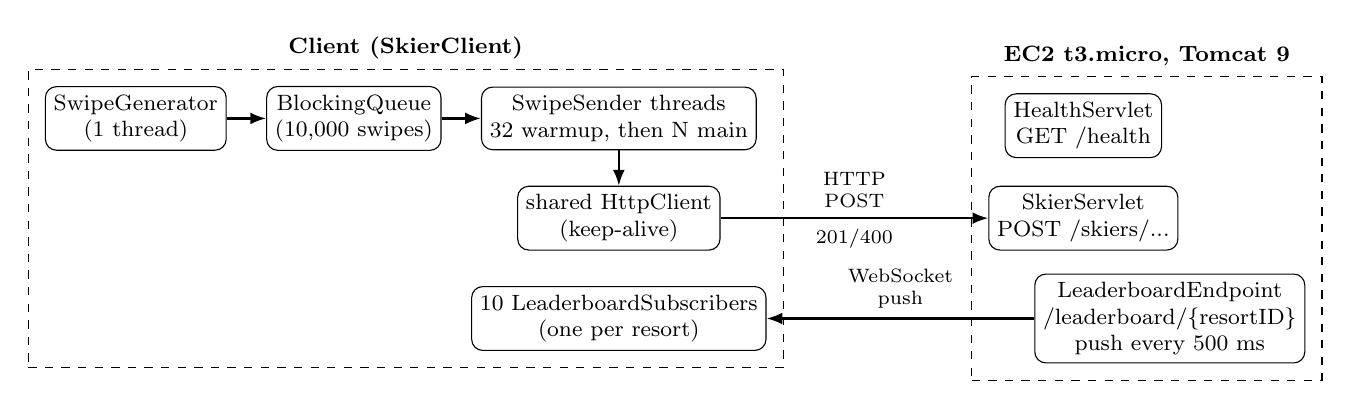
\begin{tikzpicture}[
  box/.style={draw, rounded corners, align=center, font=\footnotesize, inner sep=3pt, minimum height=0.75cm},
  arrow/.style={-{Latex[length=2mm]}, thick}]
  % client side
  \node[box] (gen) {SwipeGenerator\\(1 thread)};
  \node[box, right=0.5cm of gen] (queue) {BlockingQueue\\(10,000 swipes)};
  \node[box, right=0.5cm of queue] (senders) {SwipeSender threads\\32 warmup, then N main};
  \node[box, below=0.45cm of senders] (http) {shared HttpClient\\(keep-alive)};
  \node[box, below=0.45cm of http] (subs) {10 LeaderboardSubscribers\\(one per resort)};
  % server side
  \node[box, right=3.4cm of http] (skier) {SkierServlet\\POST /skiers/...};
  \node[box, above=0.35cm of skier] (health) {HealthServlet\\GET /health};
  \node[box, right=3.4cm of subs] (lead) {LeaderboardEndpoint\\/leaderboard/\{resortID\}\\push every 500 ms};
  % boxes around each side
  \node[draw, dashed, fit=(gen)(queue)(senders)(http)(subs), inner sep=6pt,
        label={[font=\footnotesize\bfseries]above:Client (SkierClient)}] {};
  \node[draw, dashed, fit=(health)(skier)(lead), inner sep=6pt,
        label={[font=\footnotesize\bfseries]above:EC2 t3.micro, Tomcat 9}] {};
  % arrows
  \draw[arrow] (gen) -- (queue);
  \draw[arrow] (queue) -- (senders);
  \draw[arrow] (senders) -- (http);
  \draw[arrow] (http) -- node[above, font=\scriptsize, align=center]{HTTP\\POST} node[below, font=\scriptsize]{201/400} (skier);
  \draw[arrow] (lead) -- node[above, font=\scriptsize, align=center]{WebSocket\\push} (subs);
\end{tikzpicture}
\captionof{figure}{Architecture. HTTP for swipe ingest (request/response), WebSocket for the leaderboard (server push).}
\end{center}

\subsection{Major Classes}
\textbf{Server:} \texttt{SkierServlet} is my Lab 2 servlet with stricter validation (IDs must be positive, \texttt{time} 1--360, \texttt{liftID} 1--40). It returns 201 or 400. I removed its per-request logging because logging 500K requests slows the server down. \texttt{HealthServlet} returns \texttt{\{"message":"UP"\}}. \texttt{LeaderboardEndpoint} maps each resortID to its open sessions, and one timer thread pushes a fake top 10 with a \texttt{serverTimestamp} every 500 ms. \texttt{AppListener} stops that timer on redeploy, otherwise every redeploy leaves an extra timer running. Models: \texttt{LiftRide}, \texttt{ResponseMsg}, \texttt{LeaderboardEntry}, \texttt{LeaderboardMessage}.

\textbf{Client:} \texttt{SkierClient} (\texttt{main}) runs the phases with one \texttt{SwipeGenerator} making \texttt{SwipeEvent}s, the \texttt{SwipeSender} threads and 10 \texttt{LeaderboardSubscriber}s. Part 2 adds \texttt{RequestRecord} (one CSV line) and \texttt{ThroughputChart}.

\subsection{Threading Model}
\begin{itemize}
  \item \textbf{Generation and phases:} one generator thread puts all 500,000 swipes in a \texttt{LinkedBlockingQueue} with room for 10,000. It is much faster than the network, so the senders never wait for a swipe, and the fixed size keeps memory low. In the warmup, 32 threads send 1,000 swipes each and then end. The other 468,000 swipes are split between N main-phase threads (128 on the m8azn.large, 32 on the c7g.large, 64 on the t3.micro, 512 from home, see Section~\ref{sec:experiments}). Each phase has a \texttt{CountDownLatch}, so \texttt{main} times them separately.
  \item \textbf{HTTP:} all threads share one \texttt{java.net.http.HttpClient}, which keeps connections open and reuses them. With HTTP/1.1 a connection carries one request at a time, so there is at most one connection per sending thread (32 in the warmup, then N in the main phase). Tomcat closes a kept-alive connection after 100 requests (its default \texttt{maxKeepAliveRequests}), so a 500,000-swipe run opens about 5,000 connections. The client counts them from Tomcat's \texttt{Connection: close} responses and prints them with the retries and its own CPU use, plus the WebSocket connections and reconnections.
  \item \textbf{Errors:} a failed send is retried up to 5 times, waiting 100, 200, 400, 800 and 1600 ms. Swipes that still fail are counted as failed. The counters are \texttt{AtomicInteger}s.
  \item \textbf{Part 2 metrics:} each sender times its requests with \texttt{System.nanoTime()}, the monotonic clock from Week 4, so latency isn't rounded to whole ms (the CSV timestamp stays on the wall clock). Each sender keeps its own list of \texttt{RequestRecord}s (no locking while sending), and at the end one writer writes them all to the CSV. This is the lesson from Lab 2 Exercise 3, where several writers on one file produced broken lines.
\end{itemize}

\subsection{WebSocket Connection Management}
The client opens one subscriber for each of the 10 resorts before the warmup and keeps them open for the whole run. They share one Tyrus \texttt{WebSocketContainer}. Each subscriber records its connect time, counts updates, and saves \emph{receive time $-$ serverTimestamp} as the push latency of each update. If a connection closes mid-run, \texttt{onClose} starts a thread that reconnects (up to 5 tries, 1--5 s apart). When I redeployed the server during a run, all 10 subscribers reconnected and the 128 swipes that failed during the redeploy succeeded on retry, so 0 swipes failed. On the server, \texttt{@OnClose} and \texttt{@OnError} remove the session so the map doesn't leak.

\subsection{Little's Law}
$N = X \times R$, so $X = N / R$: $N$ is the number of requests in flight (one per sender thread), $R$ is the response time (round trip) of one swipe and $X$ is the throughput (swipes per second). I measured $R$ with 200 POSTs on one kept-alive connection after a 3,000-request warmup: 0.29 ms from my m8azn.large client, 0.49 ms from my c7g.large and 0.58 ms from my t3.micro in the server's subnet, and 16 ms from my home server over Ethernet and 19 ms over Wi-Fi. \textbf{Connection overhead:} Tomcat closes each connection after 100 requests, so 1 request in 100 also opens a new connection. Inside the subnet that costs about one extra round trip, about 1\% of $R$. From home a new connection took 138 ms instead of about 19 ms, which adds about 1.2 ms per request on average (6\%). Neither explains the gap. My calculations are in Figure~\ref{fig:littles}.

\begin{center}
\screenshot[2.9in]{littles_law.jpg}{\textwidth}{my handwritten Little's Law calculations}
\captionof{figure}{My Little's Law calculations and predictions.}
\label{fig:littles}
\end{center}

\textbf{Measured vs predicted:} for my final m8azn.large run, Little's Law predicts $128 / 0.00029 = 441{,}379$ swipes/s, but I measured 22,147 swipes/s in the main phase. My client is not the limit any more (it was only 53\% busy); the t3.micro server is (95\% busy in the same setup). I predicted that ceiling from a 32-thread run, where the server was 80\% busy at 16,741 swipes/s: that is $2 \times 0.80 / 16{,}741 = 96\ \mu$s of server CPU per swipe, so at 100\% the server can do about $2 / 0.000096 = 20{,}900$ swipes/s, and with 128 threads I measured 22,147 (6\% above it: with more connections the server spent a little less CPU per swipe, 87 instead of 96~$\mu$s). Under load the requests wait at the server, so $R$ grew from 0.29 ms to $128 / X =$ 5.8 ms, and Part 2 agrees: 21,311 $\times$ 0.00570 s $=$ 121, about 128 threads. With my c7g.large client (10/14) the client was the limit instead (88--99\% CPU, 14,290 swipes/s). From home the warmup matched the prediction (1,840/s vs 2,000/s), but the main phase was limited by my home upload (about 53--61 Mbit/s).

\label{end-of-design}
% ======================= TEST RESULTS =======================
\clearpage
\section{Test Results}

\subsection{Final Runs (500,000 swipes each, 0 failed)}
\textbf{Throughput} means swipes per second: how many swipe POSTs got a 201 back each second (successful swipes $\div$ time). For example, my final Part 1 run sent 500,000 swipes in 23.07 s, so its overall throughput is 500,000 / 23.07 = 21,671 swipes/s. In the tables, ``/s'' means swipes per second. Both clients ran on EC2 in the server's subnet and used its private IP.
\begin{center}
\footnotesize
\setlength{\tabcolsep}{4pt}
\resizebox{\textwidth}{!}{\begin{tabular}{lrrrr}
\toprule
 & \textbf{Part 1 (final)} & \textbf{Part 2 (final)} & Part 1 (10/14) & Part 2 (10/14) \\
 & m8azn.large client & m8azn.large client & c7g.large client & c7g.large client \\
\midrule
Main phase threads & 128 & 128 & 32 & 32 \\
Round trip (no load) & 0.29 ms & 0.29 ms & 0.49 ms & 0.49 ms \\
Warmup (32 $\times$ 1000): time, throughput & 1.9 s, 16,486/s & 2.2 s, 14,856/s & 6.3 s, 5,076/s & 5.3 s, 6,062/s \\
Main phase: time, throughput & 21.1 s, 22,147/s & 22.0 s, 21,311/s & 32.7 s, 14,290/s & 35.2 s, 13,306/s \\
Total time, overall throughput & 23.1 s, \textbf{21,671/s} & 24.1 s, 20,734/s & 39.1 s, 12,803/s & 40.4 s, 12,361/s \\
Retries / failed swipes & 0 / 0 & 0 / 0 & 0 / 0 & 0 / 0 \\
HTTP connections reopened & 4,976 & 4,985 & not counted & not counted \\
Client CPU busy (main phase) & 53\%, 48\,$\mu$s/swipe & 49\%, 46\,$\mu$s/swipe & 88--99\% & 88--99\% \\
Ingest latency mean/median/p95/p99 & -- & 5.699 / 5.418 / 9.241 / 13.681 ms & -- & 2.57 / 2 / 5 / 10 ms \\
Ingest latency min / max & -- & 0.226 / 103.878 ms & -- & 0 / 169 ms \\
Throughput per resort & -- & 2,056--2,092/s & -- & 1,231--1,239/s \\
Leaderboard updates delivered & 470 & 480 & 780 & 811 \\
Push latency (Part 1: mean, max) & 1 ms, max 20 ms & -- & 2 ms, max 28 ms & -- \\
Push latency mean/median/p95/p99 & -- & 1.59 / 1 / 3 / 24 ms & -- & 2.23 / 2 / 6 / 12 ms \\
WebSocket connect time (avg) & 10 ms & 13 ms & 23 ms & 22 ms \\
\bottomrule
\end{tabular}}
\end{center}
With the m8azn.large client the same ingest code went from 12,803 to 21,671 swipes/s. It has 2 real cores at 5.0 GHz (the c7g.large has 2 at 2.6 GHz and the t3.micro 1 core with 2 hyperthreads), so my client stopped being the limit and the server became it. On 10/14 the latencies were rounded to whole ms; now they come from \texttt{System.nanoTime()}.

\textbf{Clock skew:} push latency compares the client clock with the server clock. All my EC2 instances sync to the Amazon Time Sync Service (the server was 6 ns off when I checked), so these push latencies are real. From home, my Windows clock kept drifting even after I synced it, so the push latency came out wrong ($-$130 ms one day and +635 ms another day). That is skew, not a bug, and it's one reason my final runs are on EC2.

\subsection{Part 1 Output (final, m8azn.large client)}
\begin{center}\screenshot{part1_output.png}{0.85\textwidth}{Part 1 client output, c7g.large}\end{center}

\subsection{Part 2 Output (final, m8azn.large client)}
\begin{center}\screenshot[5.2in]{part2_output.png}{0.85\textwidth}{Part 2 client output with the statistics}\end{center}

\subsection{Throughput Over Time (final Part 2 run, 10 second buckets)}
\begin{center}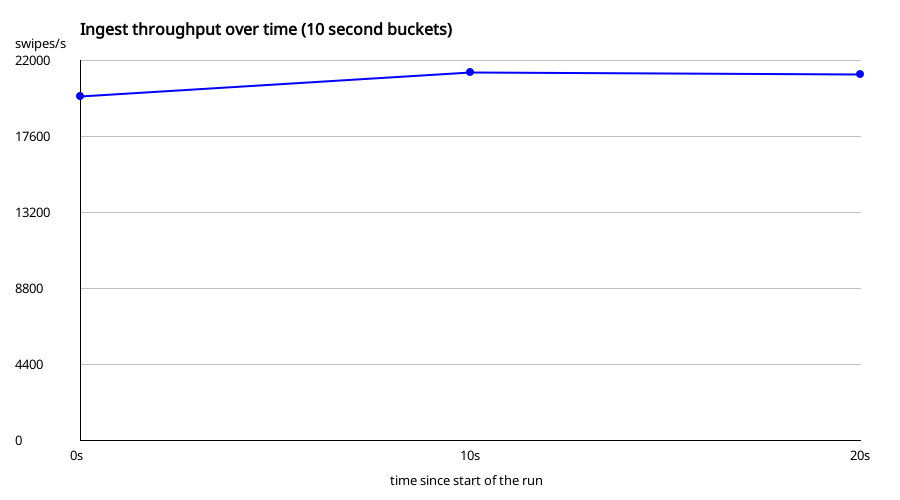
\includegraphics[width=0.8\textwidth]{images/throughput.png}\end{center}
The run is short (24.11 s), so the chart has 3 points: 19,942 / 21,335 / 21,202 swipes/s. The first bucket includes the warmup (32 threads, cold JVMs); after that the throughput stays flat because the server is at its limit. On 10/14, with the c7g.large client, throughput rose from about 7,400 to 16,100 swipes/s over a 40 s run while the client warmed up (\texttt{results/earlier\_runs/oct14\_c7g\_t3/}).

\subsection{EC2 Deployment}
\begin{center}
\screenshot[3in]{ec2_console.png}{0.85\textwidth}{EC2 console showing the server and the client instances}\\[6pt]
\screenshot[3in]{ec2_instance_details.png}{0.85\textwidth}{EC2 instance details for the server}
\end{center}
The first screenshot shows the server and the m8azn.large client running on the day of my final runs. The second one shows the server's details; its public IP changes each time the lab starts, but the private IP 172.31.36.18 stays the same. The WAR deployed on the server has the same bytecode as the server code in this repo.

\subsection{WebSocket Subscriber Receiving Leaderboard Pushes}
\begin{center}\screenshot{websocket_pushes.png}{0.85\textwidth}{Postman WebSocket connected to /leaderboard/7}\end{center}
Postman connected to \texttt{/leaderboard/7}, receiving a synthetic top 10 with a \texttt{serverTimestamp} every 500 ms.

\clearpage
\subsection{Experiments: Where Should the Client Run?}
\label{sec:experiments}
Where the client runs, and on what, decides what limits the throughput. These are my best Part 1 runs in five other setups; every run is in \texttt{results/experiment\_client\_location.txt}.
\begin{center}
\small
\begin{tabular}{lrrrr}
\toprule
 & & & Main phase & Overall \\
Client $\to$ server & Round trip & Threads & throughput & throughput \\
\midrule
Client EC2, c7g.large $\to$ my t3.micro server, best of 7 runs & 0.49 ms & 32 & 14,623/s & \textbf{13,605/s} \\
My home server (Lenovo, i7-8650U), wired $\to$ EC2 & 16 ms & 512 & 21,968/s & \textbf{12,922/s} \\
My laptop (Razer Blade 14, Ryzen 9 5900HX), wired $\to$ EC2 & 15--38 ms & 512 & 18,242/s & \textbf{11,979/s} \\
LAN test: my laptop $\to$ my home server (Tomcat, not EC2) & 0.94 ms & 64 & 41,393/s & \textbf{38,299/s} \\
Client EC2, m8azn.large $\to$ m8azn.large server (Section~\ref{sec:m8azn-server}) & 0.11 ms & 64 & 49,476/s & \textbf{45,330/s} \\
\bottomrule
\end{tabular}
\end{center}
The round trips inside AWS were measured with Java after a 3,000-request warmup. The others were measured with 200 requests from home or on the LAN.
\begin{itemize}
  \item \textbf{c7g.large client (my final setup on 10/14):} Learner Lab only allows instances up to \texttt{.large}. On Intel a \texttt{.large} is 1 core with 2 hyperthreads, but a Graviton c7g.large has 2 real cores, so I tried one in the server's subnet. Its 7 runs over two days were between 12,409 and 13,605 swipes/s. Its CPU was 88--99\% busy, so the client was the limit, while the server was about 75\% busy. The same jar on Java 21 was a bit slower (12,568--12,774 swipes/s) because its warmup was slower.
  \item \textbf{My home server (Lenovo) as the client:} its best run was wired: 12,922 swipes/s with 512 threads. From home the round trip (16 ms) sets the warmup (1,840/s, close to the 2,000/s Little's Law predicts) and my home upload (about 61 Mbit/s, full) sets the main phase, not the client CPU (63\% busy). Ethernet cut the round trip from 19 to 16 ms and made the whole run about 15\% faster than on Wi-Fi (11,226 $\to$ 12,922 swipes/s). On another day the round trip was 25 ms and the same run gave only 11,246--11,573 swipes/s.
  \item \textbf{My laptop (Razer) as the client:} its best run was 11,979 swipes/s with 512 threads, wired. Its faster CPU did not help: in my first test it got about the same as my home server (11,174/s) with 66\% of its CPU idle, which also points to my home upload (59 Mbit/s). Its round trip changed that evening (15 ms in the first test, 38 ms before the best run, during a video call), and it had 4--57 retries per run that I couldn't explain (Ethernet only, no link errors).
  \item \textbf{LAN test (technically a cheat):} to check the upload idea, I took EC2 out. I ran Tomcat on one of my machines and the client on the other, both wired to my home router (1 Gbit/s). My laptop as the client and my home server as the server gave \textbf{38,299 swipes/s} (500,000 swipes in 13.1 s), and the other way around gave 27,495 swipes/s. That is 1.3--1.8 times my final run. It is faster because nothing goes over the internet: the round trip is about 17 times shorter than from home (0.94 ms vs 16 ms), and the 1 Gbit/s link is about 16 times my home upload. The limit moved to CPU instead (my home server was 81\% busy as the server and 75\% busy as the client). The LAN run is not a valid Part 1 result because the server is supposed to run on EC2, and my home server has more CPU resources than the t3.micro. On 10/15 the t3.micro topped out at about 22,000 swipes/s (95\% CPU), so it could not keep up with 38,000 swipes/s. My final Part 1 result is 21,671 swipes/s. The LAN test shows how much faster the same code runs when the network is not the bottleneck.
\end{itemize}

\needspace{18\baselineskip}
\subsection{Experiment: m8azn.large Client and m8azn.large Server}
\label{sec:m8azn-server}
With the m8azn.large client my t3.micro server was the limit (95\% CPU). To see how fast my client can go when the server is not the limit, I launched two m8azn.large instances (2 real AMD cores at 5.0 GHz each) from an image of my server, in the same subnet: one runs Tomcat with the same WAR, the other runs the same client. This is only an experiment, because the assignment's server has to be a free-tier instance.
\begin{itemize}
  \item \textbf{Round trip:} 0.11 ms median (0.15 ms mean), vs 0.29 ms to the t3.micro.
  \item \textbf{Thread sweep (200,000 swipes, main phase):} 32 threads 38,700/s, 64 threads 39,289/s, 128 threads 32,754/s, 256 threads 31,437/s. More threads only add client CPU (48 $\mu$s per swipe at 32 threads, 63 at 256).
  \item \textbf{Best run (500,000 swipes, 64 threads):} warmup 20,369/s, main phase 49,476/s, overall \textbf{45,330 swipes/s}, 0 failed, 0 retries. The client was 93\% busy (38 $\mu$s of CPU per swipe) and the server about 53\% busy, so my client is the limit again. Four 500,000-swipe runs gave 42,276--45,330 swipes/s.
  \item \textbf{What it shows:} the same client code more than doubles its throughput when the server is not the limit (45,330 vs 21,671 swipes/s), and beats my LAN test (38,299 swipes/s).
\end{itemize}

% ===== TEMPORARY: typed Little's Law calculations to copy by hand.
% ===== This whole appendix disappears automatically once images/littles_law.jpg exists.
\IfFileExists{images/littles_law.jpg}{}{%
\clearpage
\section*{Appendix (temporary): Little's Law Calculations}
\textit{Only here so I can copy the calculations by hand. It goes away once \texttt{\detokenize{images/littles_law.jpg}} is added.}

\textbf{Formula.} $N = X \times R \;\Rightarrow\; X = N / R$, where $N$ = requests in flight (one per sender thread), $R$ = response time (round trip) of one swipe in seconds, $X$ = throughput (swipes/s). Each thread sends its requests one after another, so the time for a phase is (requests per thread) $\times\, R$.

\subsection*{1. m8azn.large client $\to$ server, my final run (R = 0.29 ms = 0.00029 s, measured median 0.29 ms, mean 0.31 ms)}
\begin{align*}
\text{Warmup: } X &= 32 / 0.00029 = 110{,}345 \text{ swipes/s} &&\text{(measured 16,486/s)}\\
\text{Warmup time} &= 1{,}000 \text{ requests} \times 0.00029 = 0.29 \text{ s} &&\text{(measured 1.94 s)}\\
\text{Main: } X &= 128 / 0.00029 = 441{,}379 \text{ swipes/s} &&\text{(measured 22,147/s)}\\
\text{Main time} &= (468{,}000 / 128) \times 0.00029 = 3{,}656 \times 0.00029 = 1.06 \text{ s} &&\text{(measured 21.13 s)}\\
\text{Total} &= 0.29 + 1.06 = 1.35 \text{ s} \;\Rightarrow\; 500{,}000 / 1.35 = 370{,}370 \text{ swipes/s} &&\text{(measured 23.07 s, 21,671/s)}
\end{align*}
\textbf{Why it is lower:} the t3.micro server is the limit, not my client (client 53\% busy, server 95\% busy). \textbf{Server ceiling} from the 32-thread run: the server was 80\% busy at 16,741 swipes/s, so $2 \times 0.80 / 16{,}741 = 0.000096$ s $= 96\ \mu$s of server CPU per swipe, and at 100\% it can do $2 / 0.000096 = 20{,}900$ swipes/s (measured with 128 threads: 22,147). \textbf{Under load:} $R = N / X = 128 /$ 22,147 $=$ 5.8 ms (not 0.29 ms). \textbf{Check with Part 2:} $N = X \times R =$ 21,311 $\times$ 0.00570 $=$ 121 $\approx 128$ threads.

\subsection*{2. c7g.large client $\to$ server, my 10/14 final run (R = 0.49 ms = 0.00049 s, measured median 0.49 ms, mean 0.51 ms)}
\begin{align*}
\text{Warmup: } X &= 32 / 0.00049 = 65{,}306 \text{ swipes/s} &&\text{(measured 5,076 $\approx$ 8\%)}\\
\text{Warmup time} &= 1{,}000 \text{ requests} \times 0.00049 = 0.49 \text{ s} &&\text{(measured 6.3 s)}\\
\text{Main: } X &= 32 / 0.00049 = 65{,}306 \text{ swipes/s} &&\text{(measured 14,290 $\approx$ 22\%)}\\
\text{Main time} &= (468{,}000 / 32) \times 0.00049 = 14{,}625 \times 0.00049 = 7.17 \text{ s} &&\text{(measured 32.7 s)}\\
\text{Total} &= 0.49 + 7.17 = 7.66 \text{ s} \;\Rightarrow\; 500{,}000 / 7.66 = 65{,}274 \text{ swipes/s} &&\text{(measured 39.1 s, 12,803/s)}
\end{align*}
\textbf{Why it is lower:} the client CPU was 88--99\% busy, so requests waited inside the client. $R = N/X = 32 / 14{,}290 = 0.00224$ s $= 2.24$ ms under load (not 0.49 ms). \textbf{Check with Part 2:} mean latency under load 2.57 ms, $N = X \times R = 13{,}306 \times 0.00257 = 34.2 \approx 32$ threads, so Little's Law holds with the real $R$. \textbf{Warmup vs main:} same 32 threads, but 5,076/s vs 14,290/s, because the JVM is still cold in the warmup (with a 50-request warmup my round-trip test gave 1.2 ms instead of 0.49 ms).

\subsection*{3. t3.micro client $\to$ server, free tier (R = 0.58 ms = 0.00058 s, measured median 0.58 ms, mean 0.61 ms)}
\begin{align*}
\text{Warmup: } X &= 32 / 0.00058 = 55{,}172 \text{ swipes/s} &&\text{(measured 4,320 $\approx$ 8\%)}\\
\text{Main: } X &= 64 / 0.00058 = 110{,}345 \text{ swipes/s} &&\text{(measured 8,602 $\approx$ 8\%)}\\
\text{Under load: } R &= N / X = 64 / 8{,}602 = 0.00744 \text{ s} = 7.44 \text{ ms}\\
\text{Check with Part 2: } N &= X \times R = 8{,}772 \times 0.00723 = 63.4 \approx 64 \text{ threads} &&\text{(mean latency 7.23 ms)}
\end{align*}
\textbf{c7g.large vs t3.micro:} main phase $14{,}290 / 8{,}602 = 1.66$ times faster with half the threads (2 real cores instead of 1 core with 2 hyperthreads).

\subsection*{4. Home server $\to$ EC2, wired (R = 16 ms = 0.016 s, measured mean 15.6--15.9 ms)}
\begin{align*}
\text{Warmup: } X &= 32 / 0.016 = 2{,}000 \text{ swipes/s} &&\text{(measured 1,840 $\approx$ 92\%)}\\
\text{Warmup time} &= 1{,}000 \text{ requests} \times 0.016 = 16.0 \text{ s} &&\text{(measured 17.4 s)}\\
\text{Main: } X &= 512 / 0.016 = 32{,}000 \text{ swipes/s} &&\text{(measured 21,968 $\approx$ 69\%)}\\
\text{Main time} &= (468{,}000 / 512) \times 0.016 = 914 \times 0.016 = 14.6 \text{ s} &&\text{(measured 21.3 s)}\\
\text{Total} &= 16.0 + 14.6 = 30.6 \text{ s} \;\Rightarrow\; 500{,}000 / 30.6 = 16{,}340 \text{ swipes/s} &&\text{(measured 38.7 s, 12,922/s)}
\end{align*}
\textbf{Connection overhead:} first request on a new connection 138 ms vs about 19 ms after it, so about $0.138 - 0.019 \approx 0.12$ s extra per thread, once. All threads connect at the same time, so each phase gets about 0.12 s longer: total $= 16.0 + 0.12 + 14.6 + 0.12 = 30.8$ s $\Rightarrow 500{,}000 / 30.8 = 16{,}234$ swipes/s (vs 16,340 without it, less than 1\% different).

\textbf{Why the main phase is lower:} $R = N/X = 512 / 21{,}968 = 0.0233$ s $= 23.3$ ms under load (not 16 ms). Upload check: $61.2 \text{ Mbit/s} \div 8 = 7.65$ MB/s, $\div\, 21{,}968$ swipes/s $= 348$ bytes per swipe, so the upload was full.

\subsection*{5. Home server $\to$ EC2, Wi-Fi (R = 19 ms = 0.019 s, measured mean 19.1--20.3 ms)}
\begin{align*}
\text{Warmup: } X &= 32 / 0.019 = 1{,}684 \text{ swipes/s} &&\text{(measured 1,605--1,629 $\approx$ 96\%)}\\
\text{Warmup time} &= 1{,}000 \text{ requests} \times 0.019 = 19.0 \text{ s} &&\text{(measured 19.9 s)}\\
\text{Main: } X &= 512 / 0.019 = 26{,}947 \text{ swipes/s} &&\text{(measured 19,014--19,801 $\approx$ 71--73\%)}\\
\text{Main time} &= (468{,}000 / 512) \times 0.019 = 914 \times 0.019 = 17.4 \text{ s} &&\text{(measured 24.6 s)}\\
\text{Total} &= 19.0 + 17.4 = 36.4 \text{ s} \;\Rightarrow\; 500{,}000 / 36.4 = 13{,}736 \text{ swipes/s} &&\text{(measured 44.5 s, 11,226/s)}
\end{align*}
\textbf{Thread sweep (main phase):} $X = N / 0.019$
\begin{center}
\begin{tabular}{rrrr}
\toprule
Threads $N$ & Predicted $N/0.019$ & Measured & Measured / predicted \\
\midrule
64 & 3,368 & 3,073 & 91\% \\
128 & 6,737 & 5,627 & 84\% \\
256 & 13,474 & 11,003 & 82\% \\
384 & 20,211 & 13,300 & 66\% \\
512 & 26,947 & 16,927 & 63\% \\
768 & 40,421 & 17,725 & 44\% \\
\bottomrule
\end{tabular}
\end{center}
\textbf{Why the main phase is lower:} solving for $R$ with the measured value gives the real round trip under load: $R = N/X = 512 / 19{,}014 = 0.0269$ s $= 26.9$ ms (not 19 ms). Upload check: $52.6 \text{ Mbit/s} \div 8 = 6.58$ MB/s, $\div\, 19{,}801$ swipes/s $= 332$ bytes per swipe, so the upload was full.

\textbf{Wired vs Wi-Fi:} only $R$ changed (19 $\to$ 16 ms), so the warmup prediction goes up by $19/16 = 1.19$ times (1,684 $\to$ 2,000). Measured: $1{,}840 / 1{,}605 = 1.15$ times.

\subsection*{6. My laptop (Razer, wired) $\to$ EC2 (R = 15 ms = 0.015 s, measured mean 14.7--15.6 ms)}
\begin{align*}
\text{Warmup: } X &= 32 / 0.015 = 2{,}133 \text{ swipes/s} &&\text{(measured 2,051 $\approx$ 96\%)}\\
\text{Warmup time} &= 1{,}000 \times 0.015 = 15.0 \text{ s} &&\text{(measured 15.6 s)}\\
\text{Main: } X &= 512 / 0.015 = 34{,}133 \text{ swipes/s} &&\text{(measured 16,058 $\approx$ 47\%, upload 59 Mbit/s full)}
\end{align*}

\subsection*{7. LAN tests (home server and laptop on the home router)}
\begin{align*}
\text{A (R = 0.00068 s): warmup } X &= 32 / 0.00068 = 47{,}059 &&\text{(measured 8,572)}\\
\text{main } X &= 64 / 0.00068 = 94{,}118 &&\text{(measured 32,383)}\\
\text{B (R = 0.00094 s): warmup } X &= 32 / 0.00094 = 34{,}043 &&\text{(measured 18,296)}\\
\text{main } X &= 64 / 0.00094 = 68{,}085 &&\text{(measured 41,393)}
\end{align*}
With sub-millisecond round trips the prediction is far too high, because the CPU becomes the limit instead of the network.
}

\end{document}
